\documentclass{article}
\usepackage[colorlinks=true]{hyperref}
\usepackage{url}
\usepackage{grffile}
\usepackage{graphicx}

\title{SumatraPDF and TeXnicCenter}
\author{Andreas Kl\"ockner}

\begin{document}
\maketitle

\section{Introduction}
While TeXnicCenter\footnote{\url{http://www.texniccenter.org/}} is one of the most popular \LaTeX\ editors in Windows environments. SumatraPDF\footnote{\url{http://blog.kowalczyk.info/software/sumatrapdf/}} is a rather unknown open-source PDF reader in comparison to the standard Adobe Reader\footnote{\url{http://get.adobe.com/de/reader/}}. However, it provides certain features, which are not available with the standard solution:
\begin{itemize}
	\item Forward and backward search,
	\item No need to close the viewer during compilation,
	\item Faster load times,
	\item Integration of the standard reader.
\end{itemize}

This document briefly explains how to set up and use especially the forward and backward search feature together with TeXnicCenter. Other \LaTeX\ editors will have similar set-up procedures. 

Please keep in mind that SumatraPDF is currently only available for Windows systems.

\section{Setup}
There is an output profile file provided with this document, which you should be able to import directly into TeXnicCenter.
\footnote{\href{run:.}{Open explorer to find SumatraPDF.tco}}
If this does not work, follow these steps in order to set up SumatraPDF to work with your TeXnicCenter installation.
\begin{enumerate}
	\item You should have installed TeXnicCenter and a \LaTeX\ distribution on your system.
	\item Retrieve and install SumatraPDF from the web: \url{http://blog.kowalczyk.info/software/sumatrapdf/}. There is also a portable version, which does not need installation into the system registries.
	\item Set up TeXnicCenter with pdf\LaTeX\ to generate synchronisation files by inserting \texttt{-synctex=-1} into the \LaTeX\ call:\\
	      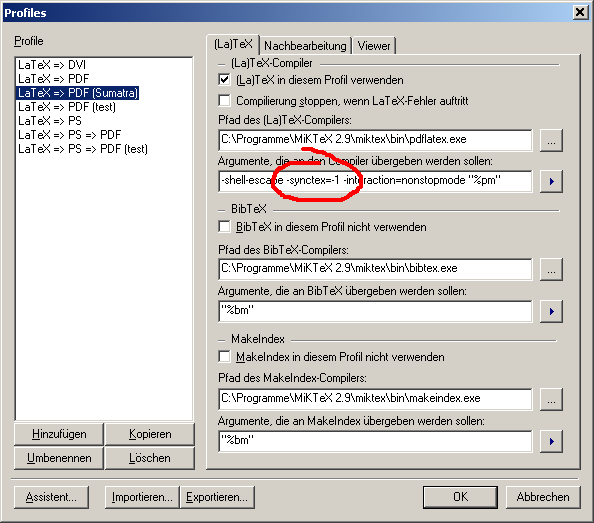
\includegraphics[width=\textwidth]{images/sumatrapdf_latex}
	\clearpage
	\item Set up TeXnicCenter to use SumatraPDF as the PDF viewer program and to use the forward search options:\\
	      Path: \texttt{SumatraPDF.exe -reuse-instance -inverse-search "\textbackslash"C:\textbackslash Programme \textbackslash TeXnicCenter\textbackslash TEXCNTR.EXE\textbackslash" /ddecmd \textbackslash"[goto('\%f','\%l')]\textbackslash""}  \\
	      DDE open command: \texttt{[Open("\%bm.pdf",0,1,1)]}  \\
	      DDE search command: \texttt{[ForwardSearch("\%bm.pdf","\%Wc",\%l,0,0,1)]} \\
	      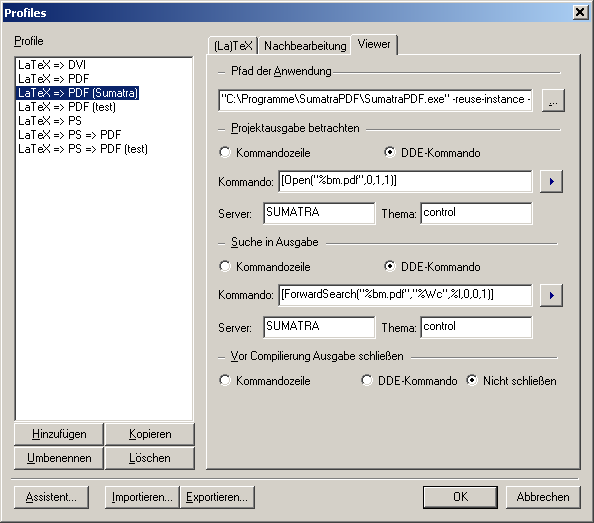
\includegraphics[width=\textwidth]{images/sumatrapdf_viewer}
	\item Your're done!
\end{enumerate}
	
\section{Use SumatraPDF}
To use SumatraPDF, you will now only need to click the 
\includegraphics[width=1em]{images/sumatrapdf_button} button or to press F5 in order to open SumatraPDF at your current cursor location in the document. A new compilation will not need to close SumatraPDF and the document will be updated automatically. Double-click an arbitrary location in the PDF document to jump to the respective location in the \LaTeX\ document. If you need Adobe Reader functionality, select "File/Open with Adobe Reader". Have fun!

\end{document}